\documentclass[tikz, border=7pt]{standalone}
\usepackage{tikz}
\usepackage{tkz-euclide}
\usepackage{amsmath}
\usepackage{amsfonts}
\usepackage{amssymb}


\newcommand\Mydiv[2]{%
$\strut#1$\kern.25em\smash{\raise.3ex\hbox{$\big)$}}$\mkern-8mu
        \overline{\enspace\strut#2}$}
\begin{document}
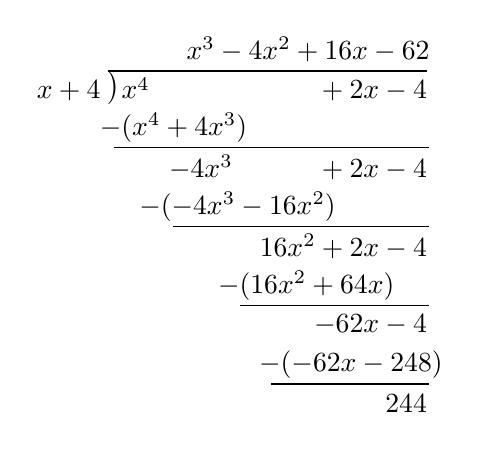
\begin{tikzpicture}

\node (c) at (0.5,3) { \Mydiv{x+4}{x^4\qquad	\qquad \qquad +2x-4}};
\draw (-1.3,2.5) node [anchor=west] {$-(x^4+4x^3)$};
\draw (-1, 2.25) -- (3,2.25);
\draw (3.1,2) node [anchor=east]{$-4x^3  \quad \qquad +2x-4$};

\draw (-0.8,1.5) node [anchor=west] {$-(-4x^3 - 16x^2)$};
\draw (-.25, 1.25) -- (3,1.25);
\draw (3.1,1) node [anchor=east]{$16x^2 +2x-4$};

\draw (0.2,0.5) node [anchor=west]{$-(16x^2+64x)$};
\draw (0.6, .25) -- (3, 0.25);
\draw (3.1,0) node [anchor=east] {$-62x- 4$};

\draw (3.3,-0.5) node [anchor=east]{$-(-62x-248)$};
\draw (1, -0.75) -- (3,-0.75);
\draw (3.1,-1) node [anchor=east] {$244$};

\draw (-0.2,3.5) node [anchor=west]{$x^3-4x^2+16x-62$};
%{$x^3-4x^2+16x-62$}


\end{tikzpicture}
\end{document}
